\subsection{THE GRADED DUALS T(M)*gr, S(M)*gr AND ∧(M)*gr}

From now on we return to the general conventions of the chapter on algebras, which will therefore be assumed (unless otherwise mentioned) to be associative and unital.

Let M be an A-module; the graded A-cogebra structures defined on T(M) (no. 1, Example 5), S(M) (no. 1, Example 6) and \(\bigwedge\) (M) (no. 1, Example 7) allow us to define canonically on the graded duals T(M)*gr, S(M)*gr and \(\bigwedge\) (M)*gr graded algebra structures of type N, by virtue of no. 2, Propositions 1 and 3 and the convention made on the graduation of the graded dual of a graded module (no. 1). Moreover, the graded algebra S(M)*gr is commutative (no. 2, Proposition 2 and Example 5) and the graded algebra \(\bigwedge\) (M)*gr is anticommutative (no. 3, Proposition 6 and Example). In \(\bigwedge\) (M)*gr every element of degree 1 is of zero square; such an element is identified with a linear form \(f\) on M and its square is the alternating bilinear form \(f \wedge f\) on M \(^{2}\) such that

\[
(f \wedge f) (x, y) = f (x) f (y) - f (y) f (x)
\]

(no. 2, Example 3).

Let \(\mathbf{N}\) be another A-module and \(u\) an A-linear mapping of \(\mathbf{M}\) into \(\mathbf{N}\) . We know that \(u\) defines canonically graded algebra homomorphisms

\[
\left\{ \begin{array}{l} \mathsf {T} (u): \mathsf {T} (\mathbf {M}) \to \mathsf {T} (\mathbf {N}) \\ \mathsf {S} (u): \mathsf {S} (\mathbf {M}) \to \mathsf {S} (\mathbf {N}) \\ \bigwedge (u): \bigwedge (\mathbf {M}) \to \bigwedge (\mathbf {N}) \end{array} \right.\tag{23}
\]

(§ 5, no. 2, § 6, no. 2 and § 7, no. 2). It is immediately verified in formula (3) of no. 1 that \(\mathsf{T}(u)\) is also a cogebra morphism. On the other hand, if \(\Delta_{\mathbf{M}}\) (resp. \(\Delta_{\mathbf{N}}\) )

denotes the diagonal mapping \(\mathbf{M} \to \mathbf{M} \times \mathbf{M}\) (resp. \(\mathbf{N} \to \mathbf{N} \times \mathbf{N}\) ), there is the relation \((u \times u) \circ \Delta_{\mathbf{M}} = \Delta_{\mathbf{N}} \circ u\) ; it follows that \(\mathbf{S}(u \times u) \circ \mathbf{S}(\Delta_{\mathbf{M}}) = \mathbf{S}(\Delta_{\mathbf{N}}) \circ \mathbf{S}(u)\)

\[
(\text { resp. } \bigwedge (u \times u) \circ \bigwedge (\Delta_ {\mathbf {M}}) = \bigwedge (\Delta_ {\mathbf {N}}) \circ \bigwedge (u)).
\]

Using the definition of coproduct in \(\mathsf{S}(\mathbf{M})\) and \(\bigwedge (\mathbf{M})\) (no. 1, Examples 6 and 7) and the functorial character of the canonical isomorphisms

\[
\mathbf {S} (\mathbf {M} \times \mathbf {M}) \rightarrow \mathbf {S} (\mathbf {M}) \otimes_ {\mathbf {A}} \mathbf {S} (\mathbf {M})
\]

and \(\bigwedge (\mathbf{M}\times \mathbf{M})\to \bigwedge (\mathbf{M})^{\mathfrak{g}}\otimes_{\mathbf{A}}\bigwedge (\mathbf{M})\) , it is seen that \(S(u)\) and \(\bigwedge (u)\) are also cogebra morphisms† (and hence in this case bigebra morphisms). It follows immediately that the graded transposes (II, § 11, no. 6) of the homomorphisms (23)

\[
\begin{array}{c} ^ {t} \mathsf {T} (u): \mathsf {T} (\mathbf {N}) ^ {* \mathrm{gr}} \to \mathsf {T} (\mathbf {M}) ^ {* \mathrm{gr}} \\ ^ {t} \mathsf {S} (u): \mathsf {S} (\mathbf {N}) ^ {* \mathrm{gr}} \to \mathsf {S} (\mathbf {M}) ^ {* \mathrm{gr}} \\ ^ {t} \bigwedge (u): \bigwedge (\mathbf {N}) ^ {* \mathrm{gr}} \to \bigwedge (\mathbf {M}) ^ {* \mathrm{gr}} \end{array}
\]

are graded algebra homomorphisms.

We now note that the dual M* of M is identified with the submodule of elements of degree 1 in T(M)*gr (resp. S(M)*gr, ∧(M)*gr). It therefore follows from the universal property of the tensor algebra (§ 5, no. 1) and the universal property of the symmetric algebra (§ 6, no. 1) that there exists one and only one graded algebra homomorphism

\[
\theta_ {\mathsf {T}}: T (M ^ {*}) \rightarrow T (M) ^ {* \mathrm{gr}}
\]

which extends the canonical injection \(\mathbf{M}^{*}\to \mathsf{T}(\mathbf{M})^{*\mathrm{gr}}\) , and one and only one graded algebra homomorphism

\[
\theta_ {\mathsf {S}}: S (M ^ {*}) \rightarrow S (M) ^ {* \mathrm{gr}}
\]

which extends the canonical injection \(\mathbf{M}^{*}\to\mathsf{S}(\mathbf{M})^{*\mathrm{gr}}\) . On the other hand, the canonical injection of \(\mathbf{M}^{*}\) in the opposite algebra to \(\bigwedge(\mathbf{M})^{*\mathrm{gr}}\) is such that the square of every element of \(\mathbf{M}^{*}\) is zero; hence (§ 7, no. 1, Proposition 1) there exists one and only one graded algebra homomorphism

\[
\theta_ {\wedge}: \bigwedge (\mathbf {M} ^ {*}) \rightarrow (\bigwedge (\mathbf {M}) ^ {* \mathrm{gr}}) ^ {\circ}
\]

which extends the canonical injection \(M^{*}\to\bigwedge(M)^{*gr.}\) . These homomorphisms are functorial: for example, for every A-module homomorphism \(u:M\to N\) , the diagram

\pandocbounded{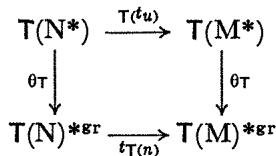
\includegraphics[keepaspectratio]{images/part004_1f4c9f33.jpg}}

is commutative, as follows immediately from the universal property of the tensor algebra (§ 5, no. 1); there are analogous commutative diagrams for \(\theta_{s}\) and \(\theta_{\wedge}\) .

We shall find the homomorphisms \(\theta_{\mathsf{T}}\) , \(\theta_{\mathsf{S}}\) and \(\theta_{\wedge}\) explicitly. For this we consider more generally a coassociative A-cogebra E with coproduct \(c\) and define by induction on \(n\) , for \(n \geqslant 2\) , the linear mapping \(c_{n}\) of E into \(\mathrm{E}^{\otimes n}\) by \(c_{2} = c\) and

\[
c _ {n} = \left(c _ {n - 1} \otimes 1 _ {\mathrm{E}}\right) \circ c.\tag{24}
\]

On the other hand we denote by \(m_{n}:A^{\otimes n}\to A\) the canonical linear mapping such that \(m_{n}(\xi_{1}\otimes\xi_{2}\otimes\cdots\otimes\xi_{n})=\xi_{1}\xi_{2}\ldots\xi_{n}\) and note that, for \(n\geqslant2\) ,

\[
m _ {n} = m \circ (m _ {n - 1} \otimes 1 _ {\mathbf {A}})\tag{25}
\]

writing \(m = m_2\) . With this notation:

Lemma 1. (i) In the associative algebra \(\mathbf{E}^* = \operatorname{Hom}_{\mathbf{A}}(\mathbf{E}, \mathbf{A})\) , the product of \(n\) elements \(u_1, u_2, \ldots, u_n\) of degree 1 is given by

\[
u _ {1} u _ {2} \dots u _ {n} = m _ {n} \circ (u _ {1} \otimes u _ {2} \otimes \dots \otimes u _ {n}) \circ c _ {n}.\tag{26}
\]

\begin{enumerate}
\def\labelenumi{(\roman{enumi})}
\setcounter{enumi}{1}
\tightlist
\item
  Suppose also that the cogebra E is graded. Then, in the graded associative algebra \(\mathbf{E}^{*\mathrm{gr}} = \operatorname{Homgr}_{\mathbf{A}}(\mathbf{E}, \mathbf{A})\) , the product of \(n\) elements \(u_1, u_2, \ldots, u_n\) of degree 1 is given by
\end{enumerate}

\[
u _ {1} u _ {2} \dots u _ {n} = m _ {n} \circ (u _ {1} \otimes u _ {2} \otimes \dots \otimes u _ {n}) \circ \delta_ {n}\tag{27}
\]

where \(\delta_n: \mathbf{E} \to \mathbf{E}^{\otimes n}\) is the linear mapping which maps each \(x \in \mathbf{E}\) to the component of \(c_n(x)\) of multidegree \((1, 1, \ldots, 1)\) .

Formula (26) is just the definition of the product in \(\mathbf{E}^*\) for \(n = 2\) ; to prove it by induction on \(n\) , observe that

\[
\begin{array}{l} u _ {1} u _ {2} \dots u _ {n} \\ \qquad = m \circ ((u _ {1} u _ {2} \dots u _ {n - 1}) \otimes u _ {n}) \circ c \\ \qquad = m \circ ((m _ {n - 1} \circ (u _ {1} \otimes u _ {2} \otimes \dots \otimes u _ {n - 1}) \circ c _ {n - 1}) \otimes u _ {n}) \circ c \\ \qquad = m \circ (m _ {n - 1} \otimes \mathrm{l} _ {\mathrm{A}}) \circ (u _ {1} \otimes u _ {2} \otimes \dots \otimes u _ {n - 1} \otimes u _ {n}) \circ (c _ {n - 1} \otimes \mathrm{l} _ {\mathrm{E}}) \circ c \\ \qquad = m _ {n} \circ (u _ {1} \otimes u _ {2} \otimes \dots \otimes u _ {n}) \circ c _ {n} \end{array}
\]

by virtue of (24), (25), II, § 3, no. 3, formula (5) and the relation

\[
u _ {n} = 1 _ {\mathbf {A}} \circ u _ {n} \circ 1 _ {\mathbf {E}}.
\]

When E is graded and the elements \(u_{i} \in E^{*gr}\) homogeneous of degree 1, then by definition for homogeneous elements \(x_{i} \in E\) ,

\[
(u _ {1} \otimes u _ {2} \otimes \dots \otimes u _ {n}) (x _ {1} \otimes x _ {2} \otimes \dots \otimes x _ {n}) = 0
\]

unless all the \(x_{i}\) are of degree 1, whence formula (27).

It follows from formulae (3), (5) and (7) of no. 1 and formula (24) that when E is taken to be one of the three graded cogebras \(\mathsf{T}(\mathbf{M})\) , \(\mathsf{S}(\mathbf{M})\) and \(\bigwedge (\mathbf{M})\) , we obtain respectively by induction on \(n\) (using the fact that the coproduct is a graded homomorphism of degree 0), for \(x_{1}, x_{2}, \ldots, x_{n}\) in M:

\[
\text { when   } \mathrm{E} = \mathrm{T} (\mathrm{M}), \quad \delta_ {n} (x _ {1} x _ {2} \dots x _ {n}) = x _ {1} \otimes x _ {2} \otimes \dots \otimes x _ {n}
\]

\[
\text { when } \mathrm{E} = \mathrm{S(M)}, \quad \delta_ {n} (x _ {1} x _ {2} \dots x _ {n}) = \sum_ {\sigma \in \mathfrak {S} _ {n}} x _ {\sigma (1)} \otimes x _ {\sigma (2)} \otimes \dots \otimes x _ {\sigma (n)}
\]

\[
\text { when } \mathrm{E} = \bigwedge (\mathrm{M}), \quad \delta_ {n} (x _ {1} x _ {2} \dots x _ {n}) = \sum_ {\sigma \in \mathfrak {S} _ {n}} \varepsilon_ {\sigma}. x _ {\sigma (1)} \otimes x _ {\sigma (2)} \otimes \dots \otimes x _ {\sigma (n)}.
\]

It suffices to note, for example when \(\mathbf{E} = \bigwedge (\mathbf{M})\) , that in the expression \(c_{n}(x_{1}x_{2}\ldots x_{n}) = (c_{n - 1}\otimes 1_{\mathbb{E}})\left(\sum (-1)^{\nu}(x_{i_1}\ldots x_{i_p})\otimes (x_{j_1}\ldots x_{j_{n - p}})\right)\) arising from formula (8) of no. 1, the only terms which can give a term of multidegree \((1,1,\dots ,1)\) are those for which \(n - p = 1\) and hence

\[
\delta_ {n} (x _ {1} x _ {2} \dots x _ {n})
\]

is the term of multidegree \((1, 1, \ldots, 1)\) in the sum

\[
\sum_ {i = 1} ^ {n} (- 1) ^ {n - i} c _ {n - 1} \left(x _ {1} \dots x _ {i - 1} x _ {i + 1} \dots x _ {n}\right) \otimes x _ {i}
\]

and this term is necessarily equal to

\[
\sum_ {i = 1} ^ {n} (- 1) ^ {n - i} \delta_ {n - 1} (x _ {1} \dots x _ {i - 1} x _ {i + 1} \dots x _ {n}) \otimes x _ {i},
\]

whence the result by the induction hypothesis.

Using Lemma 1, the product in \(\mathsf{T}(\mathbf{M})^{*\mathrm{gr}}\) of \(n\) linear forms \(x_{1}^{*}, x_{2}^{*}, \ldots, x_{n}^{*}\) of \(\mathbf{M}^{*}\) is given by

\[
\left\langle x _ {1} ^ {*} x _ {2} ^ {*} \dots x _ {n} ^ {*}, x _ {1} x _ {2} \dots x _ {n} \right\rangle = \prod_ {i = 1} ^ {n} \left\langle x _ {i} ^ {*}, x _ {i} \right\rangle\tag{28}
\]

for \(x_{i} \in \mathbf{M} (1 \leqslant i \leqslant n)\) ; the product of these \(n\) forms in \(S(M)^{*gr}\) is given by

\[
\left\langle x _ {1} ^ {*} x _ {2} ^ {*} \dots x _ {n} ^ {*}, x _ {1} x _ {2} \dots x _ {n} \right\rangle = \sum_ {\sigma \in \mathfrak {S} _ {n}} \left(\prod_ {i = 1} ^ {n} \left\langle x _ {\sigma (i)} ^ {*}, x _ {i} \right\rangle\right);\tag{29}
\]

finally, the product of these forms in \(\bigwedge (\mathbf{M})^{*\mathrm{gr}}\) is given by

\[
\langle x _ {1} ^ {*} x _ {2} ^ {*} \dots x _ {n} ^ {*}, x _ {1} x _ {2} \dots x _ {n} \rangle = \det (\langle x _ {i} ^ {*}, x _ {j} \rangle).\tag{30}
\]

In each of the three cases, we have respectively

\[
\theta_ {T} (x _ {1} ^ {*} \otimes x _ {2} ^ {*} \otimes \dots \otimes x _ {n} ^ {*}) = x _ {1} ^ {*} x _ {2} ^ {*} \dots x _ {n} ^ {*}
\]

\[
\theta_ {S} (x _ {1} ^ {*} x _ {2} ^ {*} \dots x _ {n} ^ {*}) = x _ {1} ^ {*} x _ {2} ^ {*} \dots x _ {n} ^ {*}
\]

\[
\theta_ {\wedge} (x _ {1} ^ {*} \wedge x _ {2} ^ {*} \wedge \dots \wedge x _ {n} ^ {*}) = x _ {n} ^ {*} x _ {n - 1} ^ {*} \dots x _ {1} ^ {*} = (- 1) ^ {n (n - 1) / 2} x _ {1} ^ {*} x _ {2} ^ {*} \dots x _ {n} ^ {*}
\]

and hence we deduce from (28), (29) and (30) the relations

\[
\langle \theta_ {T} (x _ {1} ^ {*} \otimes x _ {2} ^ {*} \otimes \dots \otimes x _ {n} ^ {*}), x _ {1} \otimes x _ {2} \otimes \dots \otimes x _ {n} \rangle = \prod_ {i = 1} ^ {n} \langle x _ {i} ^ {*}, x _ {i} \rangle\tag{28 bis}
\]

(in other words \(\theta_{\mathsf{T}}\) restricted to \(\mathsf{T}^2 (\mathbf{M}^*)\) is just the canonical homomorphism of II, § 4, no. 4)

\[
\langle \theta_ {\mathsf {S}} (x _ {1} ^ {*} x _ {2} ^ {*} \dots x _ {n} ^ {*}), x _ {1} x _ {2} \dots x _ {n} \rangle = \sum_ {\sigma \in \mathfrak {S} _ {n}} \left(\prod_ {i = 1} ^ {n} \langle x _ {\sigma (i)} ^ {*}, x _ {i} \rangle\right)\tag{29 bis}
\]

\[
\begin{array}{r l} (30 \text { bis}) &\langle \theta_ {\wedge} (x _ {1} ^ {*} \wedge x _ {2} ^ {*} \wedge \dots \wedge x _ {n} ^ {*}), x _ {1} \wedge x _ {2} \wedge \dots \wedge x _ {n} \rangle \\ & \qquad = (- 1) ^ {n (n - 1) / 2} \mathrm{det} (\langle x _ {i} ^ {*}, x _ {j} \rangle). \end{array}
\]

PROPOSITION 7. Let \(\mathbf{M}\) be a finitely generated projective A-module. Then the canonical homomorphisms \(\theta_{\mathsf{T}}: \mathsf{T}(\mathbf{M}^{*}) \to \mathsf{T}(\mathbf{M})^{*\mathrm{gr}}\) and \(\theta_{\wedge}: \bigwedge (\mathbf{M}^{*}) \to (\bigwedge (\mathbf{M})^{*\mathrm{gr}})^{0}\) are bijective. Also the graded dual \(\bigwedge (\mathbf{M})^{*\mathrm{gr}}\) is then equal to the dual \(\bigwedge (\mathbf{M})^{*}\) of the A-module \(\bigwedge (\mathbf{M})\) .

Suppose first that \(\mathbf{M}\) has a finite basis \((e_i)_{1\leq i\leq m}\) and let \((e_i^*)_{1\leq i\leq m}\) be the dual basis of \(\mathbf{M}^*\) (II, § 10, no. 4). Formula (28 bis) shows that, for every finite sequence \(s = (j_k)_{1\leq k\leq n}\) of \(n\) elements of the interval \([1,m]\) of \(\mathbf{N}\) ,

\[
\theta_ {\mathsf {T}} (e _ {j _ {1}} ^ {*} \otimes \dots \otimes e _ {j _ {n}} ^ {*})
\]

is the element of index \(s\) in the basis of \((\mathsf{T}^n (\mathbf{M}))^*\) , dual to the basis of \(\mathsf{T}^n (\mathbf{M})\) consisting of the \(e_s = e_{j_1}\otimes \dots \otimes e_{j_n}\) (§ 5, no. 5, Theorem 1). Hence \(\theta_{\mathsf{T}}\) is bijective.

Similarly, formula (30 bis) shows that, for every finite subset \(\mathbf{H}\) of \([1, m]\) with \(n\) elements, \((-1)^{n(n-1)/2} \theta_{\wedge}(e_{\mathrm{H}}^{*})\) (notation of §7, no. 8, Theorem 1) is the element of index \(\mathbf{H}\) in the basis of \((\bigwedge^{n}(\mathbf{M}))^{*}\) , dual to the basis of \(\bigwedge^{n}(\mathbf{M})\) consisting of the \(e_{\mathrm{H}}\) . Hence \(\theta_{\wedge}\) is bijective.

Suppose now only that M is finitely generated and projective; then M is a direct factor of a finitely generated free A-module L, so that there exist two

A-linear mappings \(M \xrightarrow{j} L \xrightarrow{p} M\) whose composition is the identity \(1_{M}\) . We deduce a commutative diagram

\pandocbounded{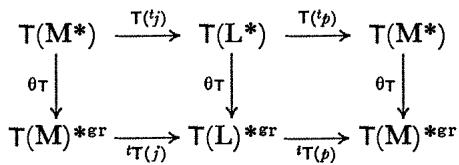
\includegraphics[keepaspectratio]{images/part004_2d3cbe02.jpg}}

and an analogous commutative diagram where \(\mathsf{T}\) is replaced by \(\bigwedge\) . The proposition then follows from the following lemma:

Lemma 2. Let

\pandocbounded{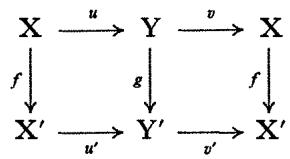
\includegraphics[keepaspectratio]{images/part004_a09507a7.jpg}}

be a commutative diagram of sets and mappings such that \(v \circ u\) and \(v' \circ u'\) are the identity mappings of \(X\) and \(X'\) respectively. Then, if \(g\) is injective (resp. surjective, resp. bijective), so is \(f\) .

u is injective since \(v \circ u\) is, hence, if g is injective, \(u' \circ f = g \circ u\) is injective and therefore f is injective. Similarly \(v'\) is surjective since \(v' \circ u'\) is; hence, if g is surjective, \(f \circ v = v' \circ g\) is surjective and therefore f is surjective.

The last assertion of Proposition 7 follows from the fact that \(\bigwedge (\mathbf{M})\) is then a finitely generated A-module (§ 7, no. 3, Proposition 6 and II, § 11, no. 6, Remark).

We now examine what can be said concerning the homomorphism \(\theta_{\mathsf{S}}\) when \(\mathbf{M}\) is projective and finitely generated. Suppose first that \(\mathbf{M}\) admits a finite basis \((e_i)_{1\leq i\leq m}\) . In the notation at the beginning of the chapter the A-module \(\mathbf{S}^n (\mathbf{M})\) admits as basis the family of elements \(e^{\alpha}\) such that \(|\alpha | = n\) . Let \(u_{\alpha}\) (for \(|\alpha | = n\) ) denote the element of index \(\alpha\) in the basis of \((\mathbf{S}^n (\mathbf{M}))^*\) dual to \((e^{\alpha})\) . The elements \(u_{\alpha}\) , for \(\alpha \in \mathbf{N}^m\) , therefore form a basis of the algebra \(\mathbf{S}(\mathbf{M})^{*\mathrm{gr}}\) and we shall obtain the multiplication table of this basis explicitly. We write

\[
u _ {\alpha} u _ {\beta} = \sum_ {\gamma \in \mathbf {N} ^ {m}} a _ {\alpha \beta \gamma} u _ {\gamma} \quad \text { with } a _ {\alpha \beta \gamma} \in \mathrm{A}.
\]

Then by definition

\[
a _ {\alpha \beta \gamma} = \langle u _ {\alpha} u _ {\beta}, e ^ {\gamma} \rangle = m ((u _ {\alpha} \otimes u _ {\beta}) (c (e ^ {\gamma}))),
\]

where \(m: \mathbf{A} \otimes \mathbf{A} \to \mathbf{A}\) defines the multiplication on \(\mathbf{A}\) and \(c\) is the coproduct of \(\mathsf{S}(\mathbf{M})\) . In other words, \(a_{\alpha \beta \gamma}\) is just the coefficient of \(e^{\alpha} \otimes e^{\beta}\) when \(c(e^{\gamma})\) is written in terms of the basis of \(\mathsf{S}(\mathbf{M})\otimes \mathsf{S}(\mathbf{M})\) consisting of the \(e^{\xi}\otimes e^{\eta}\) , where \(\xi\) and \(\eta\) run through \(\mathbf{N}^m\) . But since \(c\) is an algebra homomorphism,

\[
c (e ^ {\gamma}) = \prod_ {i = 1} ^ {m} (c (e _ {i})) ^ {\gamma_ {i}} = \prod_ {i = 1} ^ {m} (e _ {i} \otimes 1 + 1 \otimes e _ {i}) ^ {\gamma_ {i}}
\]

by formula (4) of no. 1; this gives

\[
c (e ^ {\gamma}) = \sum_ {\xi + \eta = \gamma} (\xi , \eta) e ^ {\xi} \otimes e ^ {\eta}\tag{31}
\]

where we write

\[
((\xi , \eta)) = \prod_ {i = 1} ^ {n} \frac {(\xi_ {i} + \eta_ {i}) !}{\xi_ {i} ! \eta_ {i} !} \quad (\text { cf.   } \S 10, \text {   no.   } 4, \text {   formula   (18) }).\tag{32}
\]

Hence we obtain the multiplication table

\[
u _ {\alpha} u _ {\beta} = ((\alpha , \beta)) u _ {\alpha + \beta}.\tag{33}
\]

On the other hand, if \((e_i^*)_{1\leq i\leq m}\) is the basis of \(\mathbf{M}^*\) , dual to \((e_i)\) , it follows from formula (29 bis) that, for all \(\alpha \in \mathbf{N}^m\) ,

\[
\theta_ {S} (e ^ {* \alpha}) = \alpha ! u _ {\alpha}\tag{34}
\]

in the notation of § 6, no. 6. Hence the homomorphism \(\theta_{\mathsf{S}}\) is bijective if and only if the \(\alpha!u_{\alpha}\) form a basis of \(\mathsf{S}(\mathbf{M})^{*\mathrm{gr}}\) , or also if the elements \(\alpha!1\) are invertible.

PROPOSITION 8. Suppose that the ring A is an algebra over the field Q of rational numbers; then, for every finitely generated projective A-module M, the homomorphism

\[
\theta_ {\mathsf {S}}: S (M ^ {*}) \rightarrow S (M) ^ {* \mathrm{gr}}
\]

is bijective.

It amounts to proving this when M is finitely generated and free; we pass from this to the general case using Lemma 2 as in the proof of Proposition 7.

Remark. Let M be an A-module and \(\rho: \mathbf{A} \to \mathbf{B}\) a commutative ring homomorphism. Then there is a commutative diagram of graded B-algebra homomorphisms

\[
\begin{array}{l} \mathsf {T} ((\mathbf {M} ^ {*}) _ {(B)}) \longrightarrow (\mathsf {T} (\mathbf {M}) ^ {* \mathrm{gr}}) _ {(B)} \\ \mathsf {T} (\upsilon_ {\mathbf {M}}) \Biggl \downarrow \qquad \qquad \qquad \qquad \qquad \qquad \qquad \qquad \qquad \Biggl \downarrow \upsilon_ {\mathbf {T} (\mathbf {M})} \\ \mathsf {T} ((\mathbf {M} _ {(B)}) ^ {*}) \xrightarrow [ \theta_ {\mathsf {T}} ]{} \mathsf {T} (\mathbf {M} _ {(B)}) ^ {* \mathrm{gr}} \end{array}
\]

where the first row is a homomorphism composed of the homomorphism \(\theta_{\mathsf{T}}\otimes 1_{\mathsf{B}}\colon \mathsf{T}(\mathbf{M}^{*})\otimes_{\mathbf{A}}\mathbf{B}\to \mathsf{T}(\mathbf{M})^{*\mathrm{gr}}\) and the canonical isomorphism

\[
\mathsf {T} ((\mathbf {M} ^ {*}) _ {(\mathbf {B})}) \rightarrow \mathsf {T} (\mathbf {M} ^ {*}) \otimes_ {\mathbf {A}} \mathbf {B}
\]

(§ 5, no. 3, Proposition 5). It is immediately verified, using formula (28) and the definition of the homomorphism \(\upsilon_{\mathbf{E}}\) (II, § 5, no. 4), that this diagram is commutative. When \(\mathbf{M}\) is a finitely generated projective A-module, \(\mathbf{M}_{(\mathbf{B})}\) is a finitely generated projective B-module (II, § 5, no. 1, Corollary to Proposition 4) and all the homomorphisms of the above diagram are bijective (Proposition 7 and II, § 5, no. 4, Proposition 8). There are analogous commutative diagrams with \(\mathsf{T}\) replaced by \(\mathsf{S}\) or \(\bigwedge\) ; the diagram for \(\bigwedge\) also consists of bijective homomorphisms when \(\mathbf{M}\) is projective and finitely generated (Proposition 7); if further \(\mathbf{A}\) is an algebra over \(\mathbf{Q}\) , the diagram for \(\mathsf{S}\) also consists of bijective homomorphisms (Proposition 8).

